% This chapter is pretty flowery, but so am I *shrug*
\section{The Decade for Surveys}

One would be hard-pressed to find a better time to be working in astronomy than at this moment.
Amazing new instruments are coming online that are pushing the boundaries of what can be observed, giving astronomers a deluge of data to explore and new secrets of the universe to unlock.
For engineers, every new instrument starts as a question, “What is possible?”
Every year the answer changes as technology progresses, giving astronomers more compute power, more sensitivity, and lower costs.

This decade is especially exciting with the deployment of a slew of powerful new instruments.
Specifically, we are seeing an emphasis on survey instruments, mapping out the sky across the entire EM spectrum.
These types of experiments are not proposal-based where one would request to look at some interesting object, instead relying on the community at large to explore the data, searching for patterns, outliers, and really anything interesting.
This is well-motivated, as most major discoveries in astronomy were serendipitous.
Having such a large volume of data across parameter space enables discovery of the unexpected, assuming we are prepared~\cite{norrisDiscoveringUnexpectedAstronomical2017}.
Additionally, surveys democratize science by enabling everyone to explore the rich datasets, instead of allowing only a select few whose proposals were accepted to have access to high-quality data.
All this is to say that surveys are a key tool in modern astronomy and are consistently ranked among the highest priority in science funding~\cite{nationalacademiesofsciencesPathwaysDiscoveryAstronomy2023}.

In the optical, the Vera Rubin Observatory in Chile will soon conduct a massive all-sky survey~\cite{biancoOptimizationObservingCadence2021}, with a projected first light in July 2025.
The recently launched SPHEREx satellite~\cite{crillSPHERExNASAsNearinfrared2020} will survey the near infrared and will be starting its survey soon.
In the radio, the VLA Sky Survey (VLASS)~\cite{lacyKarlJanskyVery2020} is ongoing, imaging the whole sky visible to the VLA in New Mexico.
This experiment builds off the success of previous VLA-based surveys\footnote{Which are some of the most scientifically successful experiments that the VLA has performed}, further improving sensitivity and resolution.
While continuing to be successful, the speed at which VLASS images the sky is comparatively very slow.
Rubin images \qty{10}{deg^2} every \qty{15}{\s} or \qty{2400}{deg^2/hr} (during the nighttime).
SPHEREx will survey the entire sky once every six months, or a speed of \qty{5}{deg^2/hr}.
Finally, VLASS operates at about \qty{0.01}{deg^2/hr}, while splitting time between the survey and other planned observations.
Even though VLASS (and previous radio surveys) are very successful, they are being executed on instruments poorly optimized for surveys.

This is where the Deep Synoptic Array 2000 (DSA-2000)~\cite{hallinanDSA2000RadioSurvey2019} comes in.
Rather than using existing radio telescopes to survey the sky, we propose a bespoke survey instrument to match the scale and cadence of surveys from other wavelengths.
This will result in a massive legacy dataset that will be transformative in radio astronomy and produce enough data to keep astronomers busy for decades to come.

\section{Designing A Survey Instrument}

In the design of a survey instrument, the key metric is the speed at which we can create images of the sky.
The faster we can make high-sensitivity maps, the faster we can get these maps in the hands of astronomers to do science.
We can quantify this measure via survey speed, defined as the time required to map one patch of sky down to some fixed noise level
\begin{equation}
        \text{SS}~(\text{deg}^2/\text{hr}) \approx 1.217\eta_a\Delta_\nu\left[\frac{\lambda S_\nu N D}{T_\text{Sys}}\right]^2
\end{equation}
This equation for the survey speed of reflector-based radio telescope arrays (derived in \autoref{sec:survey_speed}), depends on the number of antennas $N$, the system noise temperature $T_\text{Sys}$, the diameter of the dishes $D$, the aperture efficiency of the dishes $\eta_a$, the observation wavelength $\lambda$, the integration bandwidth $\Delta_\nu$, and the desired $1\sigma$ flux density $S_\nu$ in Jy.
In essence, this metric combines the sensitivity of the instrument with how much of the sky it can see.
One could also just ask about that sensitivity, given by
\begin{equation}
    S_\nu~(\mu\text{Jy @ 1 hr}) \approx 1852\frac{T_\text{Sys}}{\eta_aD^2N\sqrt{\Delta_{\nu\text{(GHz)}}}}
\end{equation}
which gives the RMS noise in $\mu$Jy in one hour of integration.
The ideal instrument would have a minimal noise and a large collecting area, which corresponds to a high survey speed.

\begin{figure}[ht!]
    \centering
    \includestandalone[mode=buildnew]{figures/dsa2000_compare}
    \caption{Comparison of radio telescopes at \qty{1.4}{\GHz} in survey speed and sensitivity}
    \label{fig:dsa2000_compare}
\end{figure}

Using these metrics, we can compare the planned DSA-2000 performance against other planned and deployed instruments.
DSA-2000 will be composed of 2000, \qty{5}{\m} dishes operating at an aperture efficiency of about \num{0.7}, observing from \SIrange{0.7}{2}{\GHz} with a system noise temperature of about \qty{25}{\K}.
For this comparison, we will look at DSA-110~\cite{raviDSA110OverviewFirst2023}, ASKAP~\cite{hotanAustralianSquareKilometre2021}, MeerKAT~\cite{jonasMeerKATRadioTelescope2018a}, CHORD~\cite{vanderlindeCanadianHydrogenObservatory2019}, 
VLA~\cite{VLAObservationalStatus}, and ngVLA~\cite{NgVLAPerformanceEstimates}, shown in \autoref{fig:dsa2000_compare}.
With these results, we can see that the DSA-2000 outperforms all instruments in this band in survey speed, with only ngVLA having higher sensitivity.
This is not too surprising as the ngVLA is a multi-billion dollar project with large, cryogenically cooled receivers.
If we quantify the science output of these instruments as proportional to their survey speed\footnote{A somewhat dubious claim, but good enough for this exercise}, and then try to predict science per dollar, we see a very different story.

The construction costs for a radio telescope array can be broken down into two major chunks: the processing hardware and the antennas themselves.
For an $N$-antenna array, the cost of the compute scales with $N^2$.
We will ignore operation cost and everything else just so we can get a grasp on the design-space.
To keep costs low, it would seem that we would want to keep $N$ low, but our survey speed \textit{increases} by $N^2$, so these are certainly at odds.
Currently, compute is relatively inexpensive for the kind of processing we need to do, at least compared to the cost of the antenna hardware itself.
Our current estimates for DSA-2000 put the cost of the compute (again ignoring power, installation, operations, etc.) at around \$20M for 2000 antennas.
The antennas cost about \$30k each, for a total of \$60M before trenching, installation, etc.
Compare this to  ngVLA's much larger, cryogenically cooled antennas, which cost about \$7M each.

% \begin{figure}[ht!]
%     \centering
%     \includestandalone[mode=buildnew]{figures/ss_per_dollar}
%     \caption[Survey speed for fixed budget]{Survey speed for a fixed budget of \$100M}
%     \label{fig:ss_per_dollar}
% \end{figure}

% Designing a sensitive antenna can be expensive, so an important question is how to spend your money.
% If you designed an expensive, cryogenic receiver like the ngVLA, you will certainly win in sensitivity.
% However, at some point, one could imagine that many cheap antennas might beat the expensive solution at scale.
% Again, assuming a fixed compute cost scaling, the price per antenna (and the sensitivity of each antenna) is really what matters.
% We can better visualize this by looking at the sensitivity of a few instruments, given a fixed budget of \$100M, shown in \autoref{fig:ss_per_dollar}.

% In \autoref{fig:ss_per_dollar}, we include a point for DSA-10~\cite{koczDSA10PrototypeArray2019}, a last-generation pathfinder instrument.
% DSA-10 had a system temperature of around \qty{60}{\K}, but was relatively inexpensive to build.
% DSA-110 was a progression on this design, with massive improvements in the LNA~\cite{weinrebLowNoiseAmplifier2021} reducing the system noise to \qty{25}{\K}.
% Finally, we see DSA-2000 at the top of the plot.
% DSA-2000's antennas are pricier, which reduces the number that one could build with a fixed budget, but the tradeoff still improved survey speed per dollar.
% For comparison, we include 15 ngVLA antennas, which is about what you could build with this fixed budget.

Matching the ngVLA, we could add cryogenics to cool the DSA-2000 receiver to \qty{20}{\K}, which would cost about \$100k per antenna~\cite{daddarioAdvancedCryocoolersNext2017}.
Simulations predict this will reduce our system noise temperature by \qty{7}{\K} to \qty{18}{\K}, as cooling only impacts the feed and LNA and there are still other sources of noise (the sky, spillover noise, etc. See \autoref{fig:tsys_contributions}).
If each antenna costs around \$30k, we quadruple the cost of each antenna, while not even doubling the survey speed.% (\qty{32}{deg^2/hr} to \qty{63}{deg^2/hr}).

All of this leads to the conclusion that if you can build a high-performance, cheap antenna, build lots of them!
And the key to an inexpensive antenna is not using cryogenics.
As survey speed scales with $T_\text{Sys}^{-2}$, any reduction in system noise will dramatically increase the science per dollar of the instrument.
The strong impact of reducing noise then motivates the work in this thesis, where reducing the system noise by even \qty{1}{\K} would save about \$1M in cost to maintain survey speed.
Of all the contributions to $T_\text{Sys}$, currently the LNA is the largest (as shown in \autoref{fig:tsys_contributions}) which suggests where to spend effort to maximize the impact on the science.

\begin{figure}[ht!]
    \centering
    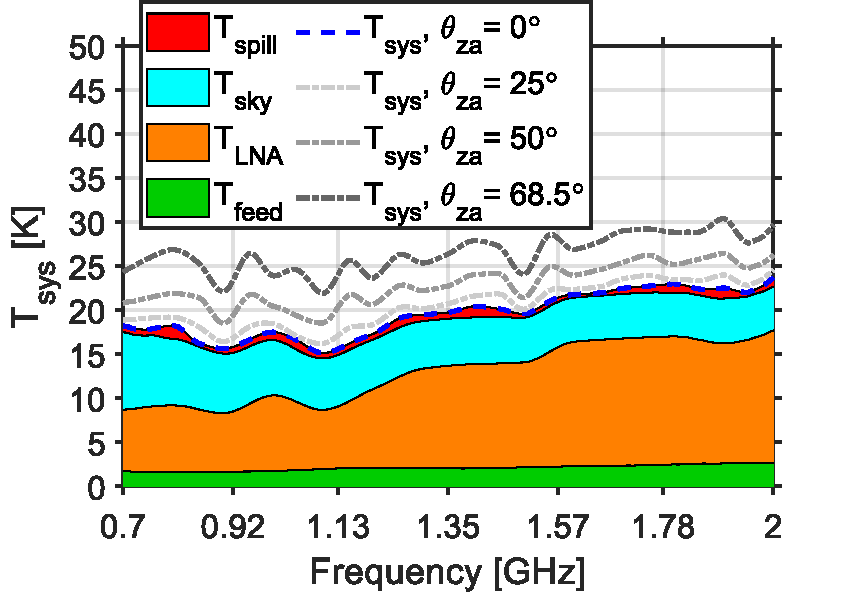
\includegraphics[width=0.8\textwidth]{figures/DSA2000_Tsys.pdf}
    \caption[DSA-2000 system noise temperature contributions]{DSA-2000 system noise temperature contributions. Reproduced from~\cite{flygareWidebandLowLossFeed2024} with permission from J. Flygare.}
    \label{fig:tsys_contributions}
\end{figure}

If it is so obvious to build a large $N$ telescope, a reasonable question would be, “why haven't people done this before?”
To answer this, we need to discuss a bit more about radio telescope interferometers.

Radio telescopes were historically built using a single, large aperture.
A large collecting area increases sensitivity and resolution, but the cost of building a large reflector with diameter $D$ is $\propto D^{2.5-2.7}$~\cite{belleScalingRelationshipTelescope2004}.
Additionally, there are practical upper limits on the size of a reflector one could build, with the largest single-dish antenna being the FAST telescope in China at \qty{500}{\m} in diameter, with a \qty{300}{\m} effective aperture.
At a typical observation frequency of \qty{1.4}{\GHz}, the diffraction-limited resolution of FAST is \qty{3}{arcmin}.
Compare this with a modest optical observatory such as Keck, with a \qty{10}{\m} mirror, where they achieve an angular resolution of better than \qty{0.05}{arcsec}.

To overcome this resolution shortcoming, the concept of radio interferometry was developed by Ruby Payne-Scott and Joseph Pawsey in the 1940s.
They used the interference pattern produced by combining radio signals reflecting off the ocean with a receiver on top of a cliff to pinpoint emission from sunspots.
This essentially provided them with the angular resolution of a telescope the size of the distance from their antenna to the image of their antenna in the ocean.
This concept was further developed by Martin Ryle and Antony Hewish in the 50s, where they used Earth's rotation to synthesize a massive equivalent aperture.
This technique is so powerful, it was part of Ryle and Hewish's Nobel Prize in Physics in 1974\footnote{Which, notably, did not include Jocelyn Bell who actually discovered the first pulsar to which the Prize was attributed}.
Modern aperture synthesis uses a combination of spatially distributed antennas and Earth rotation to synthesize a single massive telescope.
Very long baseline interferometry (VLBI) has receivers all over the world to synthesize an Earth-sized telescope, used to create the first images of a black hole~\cite{eventhorizontelescopecollaborationFirstM87Event2019}.

The radio interferometer imaging procedure starts with the coherent combination of the time-averaged product of signals from pairs of antennas.
As the signal from the sky is essentially incoherent noise, this result is a statistical correlation product between antennas.
The surprising result is that there exists a relationship between the collection of all these correlation products (known as visibilities) and the image of the sky.
This relationship is known as the van Cittert-Zernike theorem\footnote{Using a small angle approximation, which results in the Fourier relationship} and states
\begin{equation}
    V(\mathbf{r}_1,\mathbf{r}_2) \approx \iint_{-\infty}^{\infty}I(l,m)e^{-2\pi j(ul+vm)}dldm = \mathcal{F}\{I(l,m)\}
\end{equation}
where $V(\mathbf{r}_1,\mathbf{r}_2)$ is the visibility or mutual spatial coherence function given by the time average product of the received signal (electric field) from the pair of antennas at two points in space ($\mathbf{r}_1$ and $\mathbf{r}_2$)
\begin{equation}
    V(\mathbf{r}_1,\mathbf{r}_2) = \langle E(\mathbf{r}_1)E(\mathbf{r}_2)^*\rangle
\end{equation}
and $u$ and $v$ are the spatial differences between the two points\footnote{Ignoring changes in height $z$, which is something you might want to consider~\cite{cornwellProjectionNewAlgorithm}}
\begin{equation}
    \mathbf{r}_1 - \mathbf{r}_2 = \mathbf{u} = (x_1-x_2, y_1 - y_2) = (u,v)
\end{equation}
and $I(l,m)$ is the intensity distribution (image) of the sky in a direction-cosine reference frame.
All of this is to say that the inverse Fourier transform of the visibilities gives us the image of the sky!
%
\begin{figure}[ht!]
    \centering
    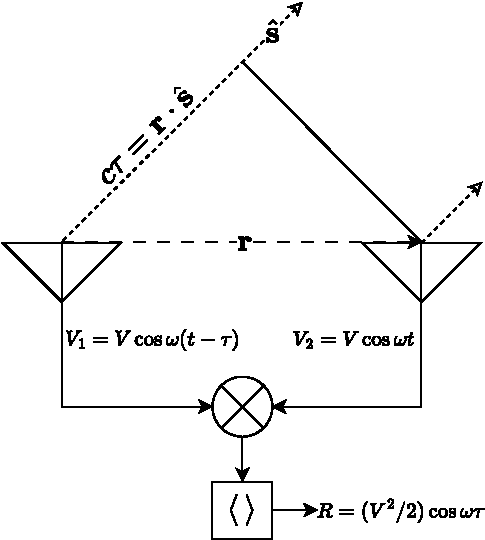
\includegraphics[width=0.5\textwidth]{figures/radio_interferometer.pdf}
    \caption{Diagram of a radio interferometer}
    \label{fig:interferometer_diagram}
\end{figure}

A problem then arises from the fact that we have not continuously sampled all the points in $u$ and $v$ as we have a discrete number of antennas and therefore a finite number of visibilities.
Not only that, but there is a maximum distance that we can separate antennas.
Combining these two shortcomings, we essentially image the sky through a diffraction-limited, shattered mirror.
This imaging procedure is shown in \autoref{fig:radio_imaging} as Fourier pairs, where a sparse sampling of the Fourier-domain of the true image of the sky results in the measured, dirty image.
The dirty image itself is not usable for science, so we must attempt to recover the true image algorithmically.
However, due to the sparse sampling of the $uv$ plane, this is an ill-posed inverse problem and does not have a simple solution.
Various optimization-based strategies are used for this, perhaps the most popular being an iterative blind deconvolution algorithm called CLEAN~\cite{hogbomApertureSynthesisNonRegular1974}.

\begin{figure}[ht!]%
    \centering
    \setlength{\tabcolsep}{1pt} % spacing between columns
    %\renewcommand{\arraystretch}{1} % spacing between rows
    \begin{tabular}{ccccc}
        \captionsetup{position=top}
        \subfloat[True Image]{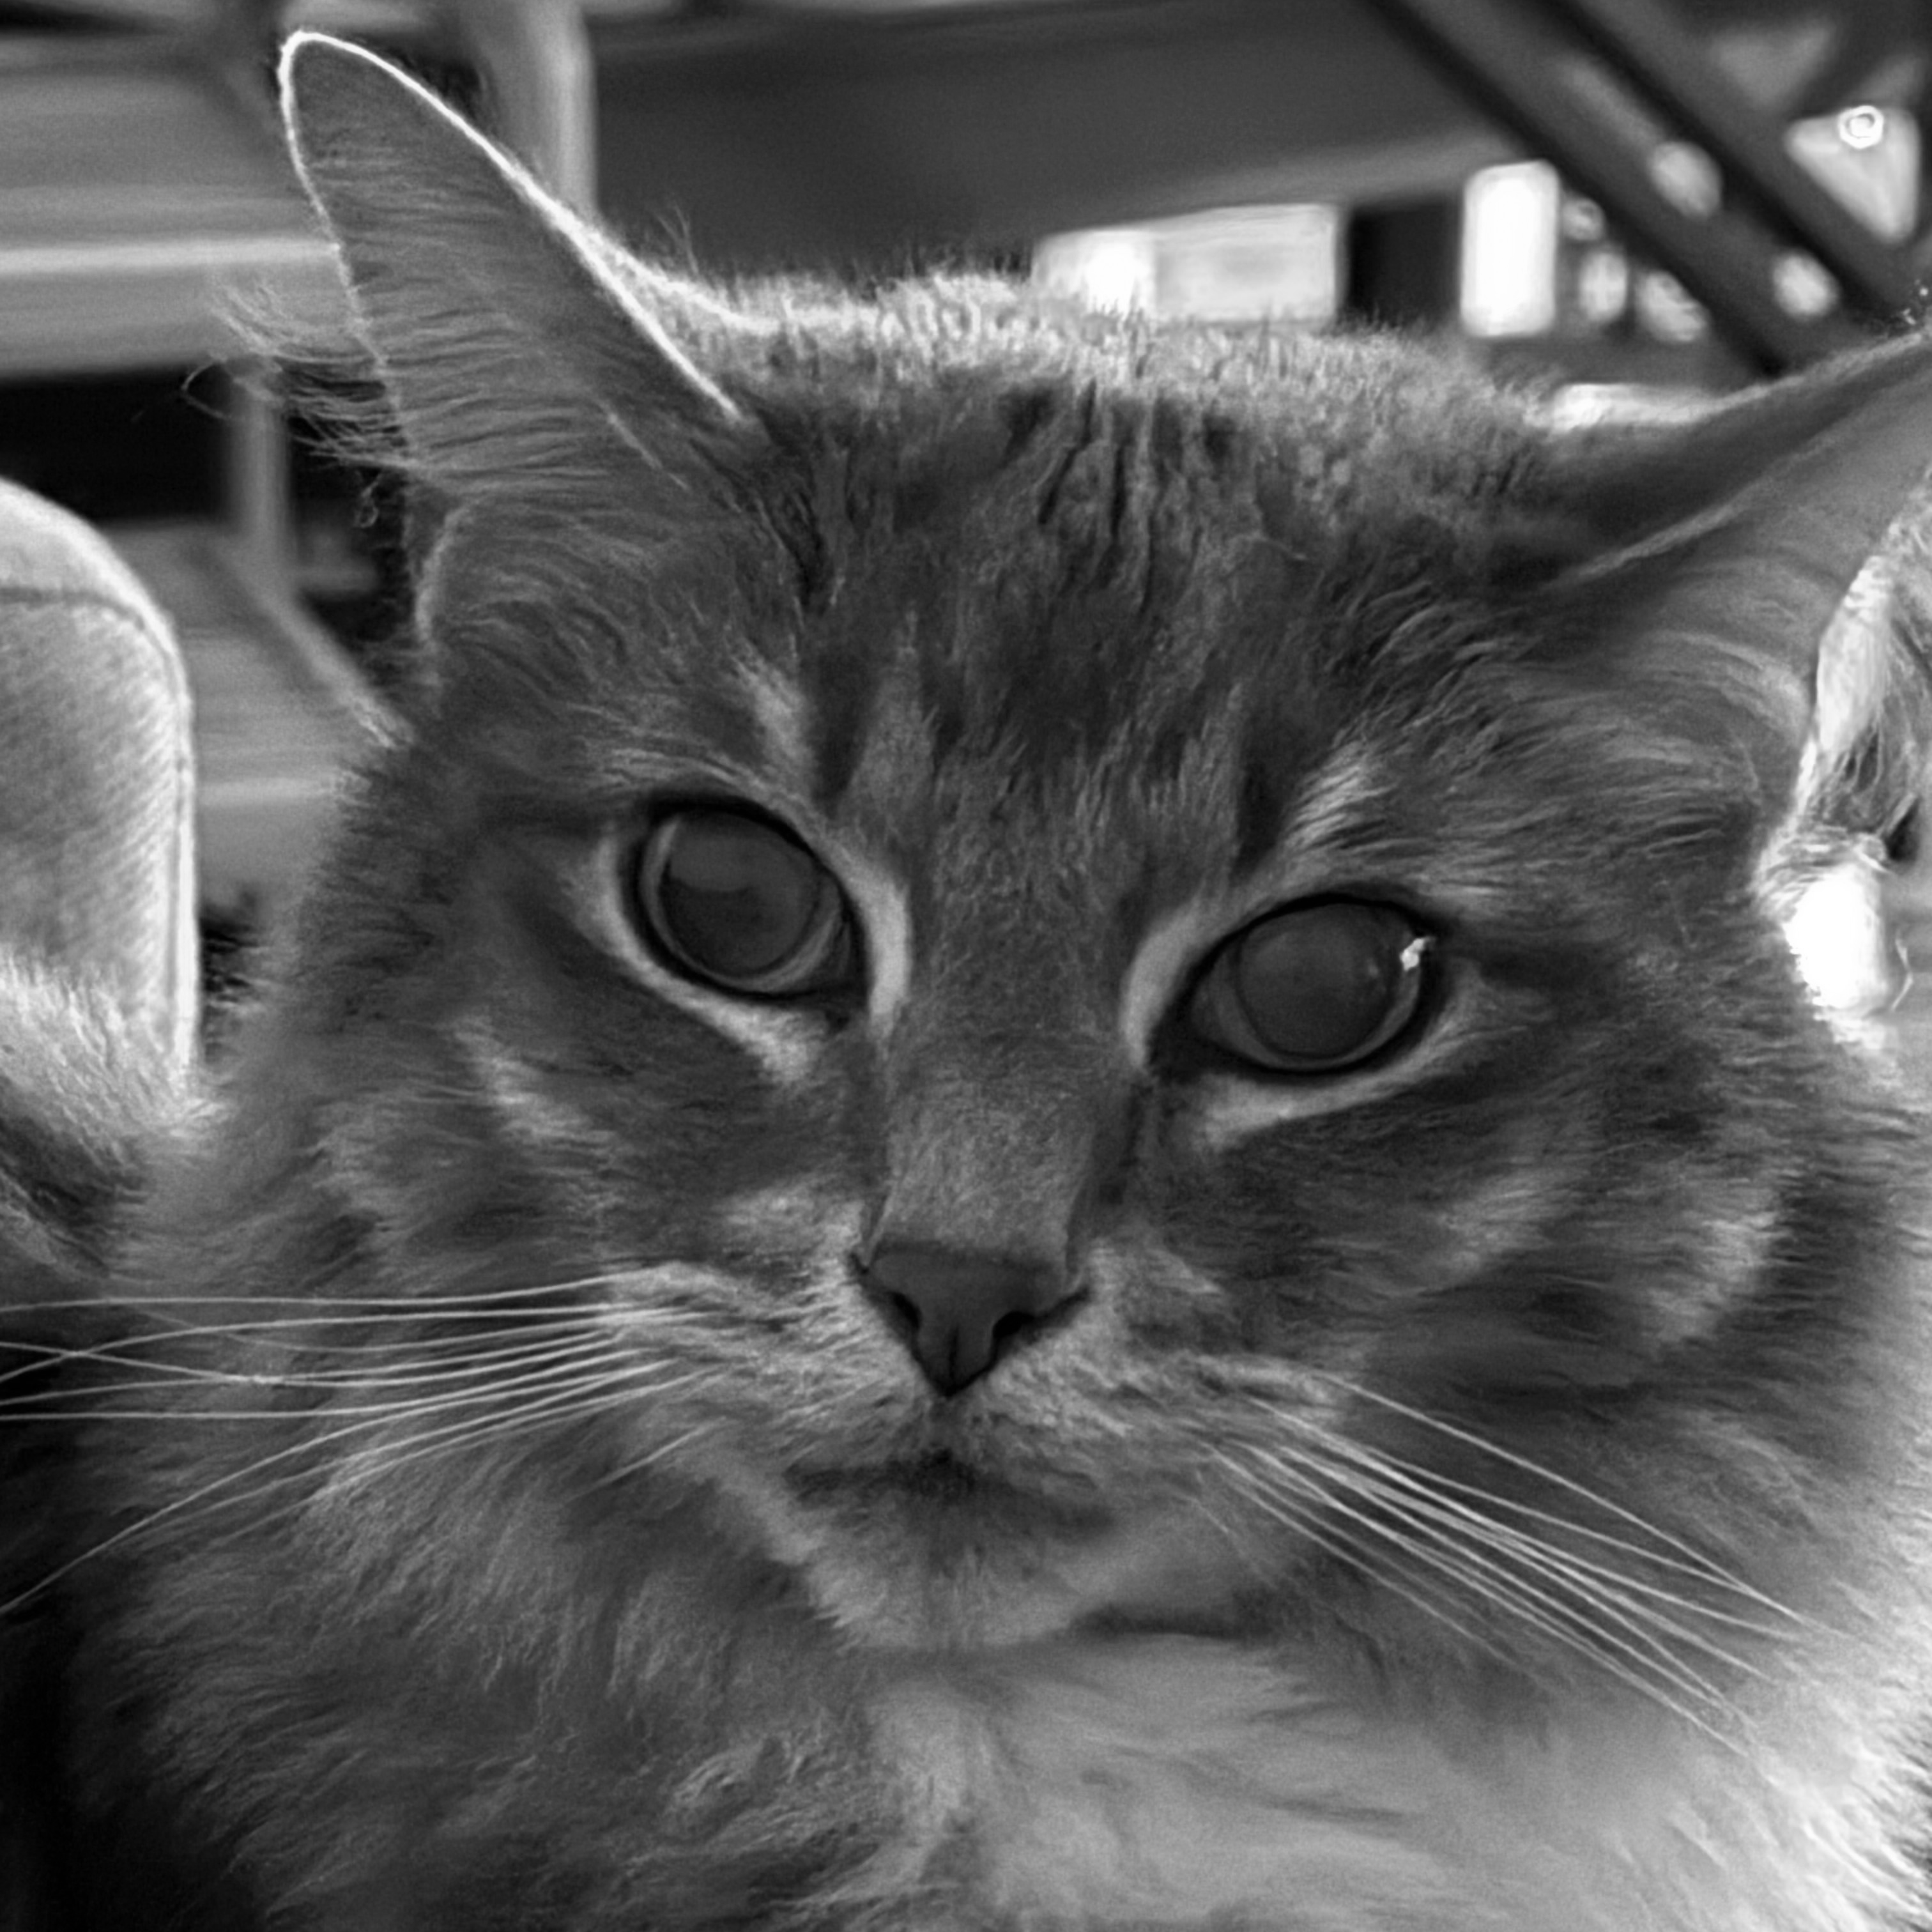
\includegraphics[height=4cm]{figures/rocket.png}} &
        \raisebox{-2.2cm}{$\scalebox{1.5}{$\circledast$}$} &
        \captionsetup{position=top}
        \subfloat[Point-Spread Function]{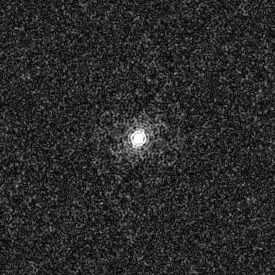
\includegraphics[height=4cm]{figures/psf.png}} &
        \raisebox{-2.2cm}{$\scalebox{1.5}{$=$}$} &
        \captionsetup{position=top}
        \subfloat[Dirty Image]{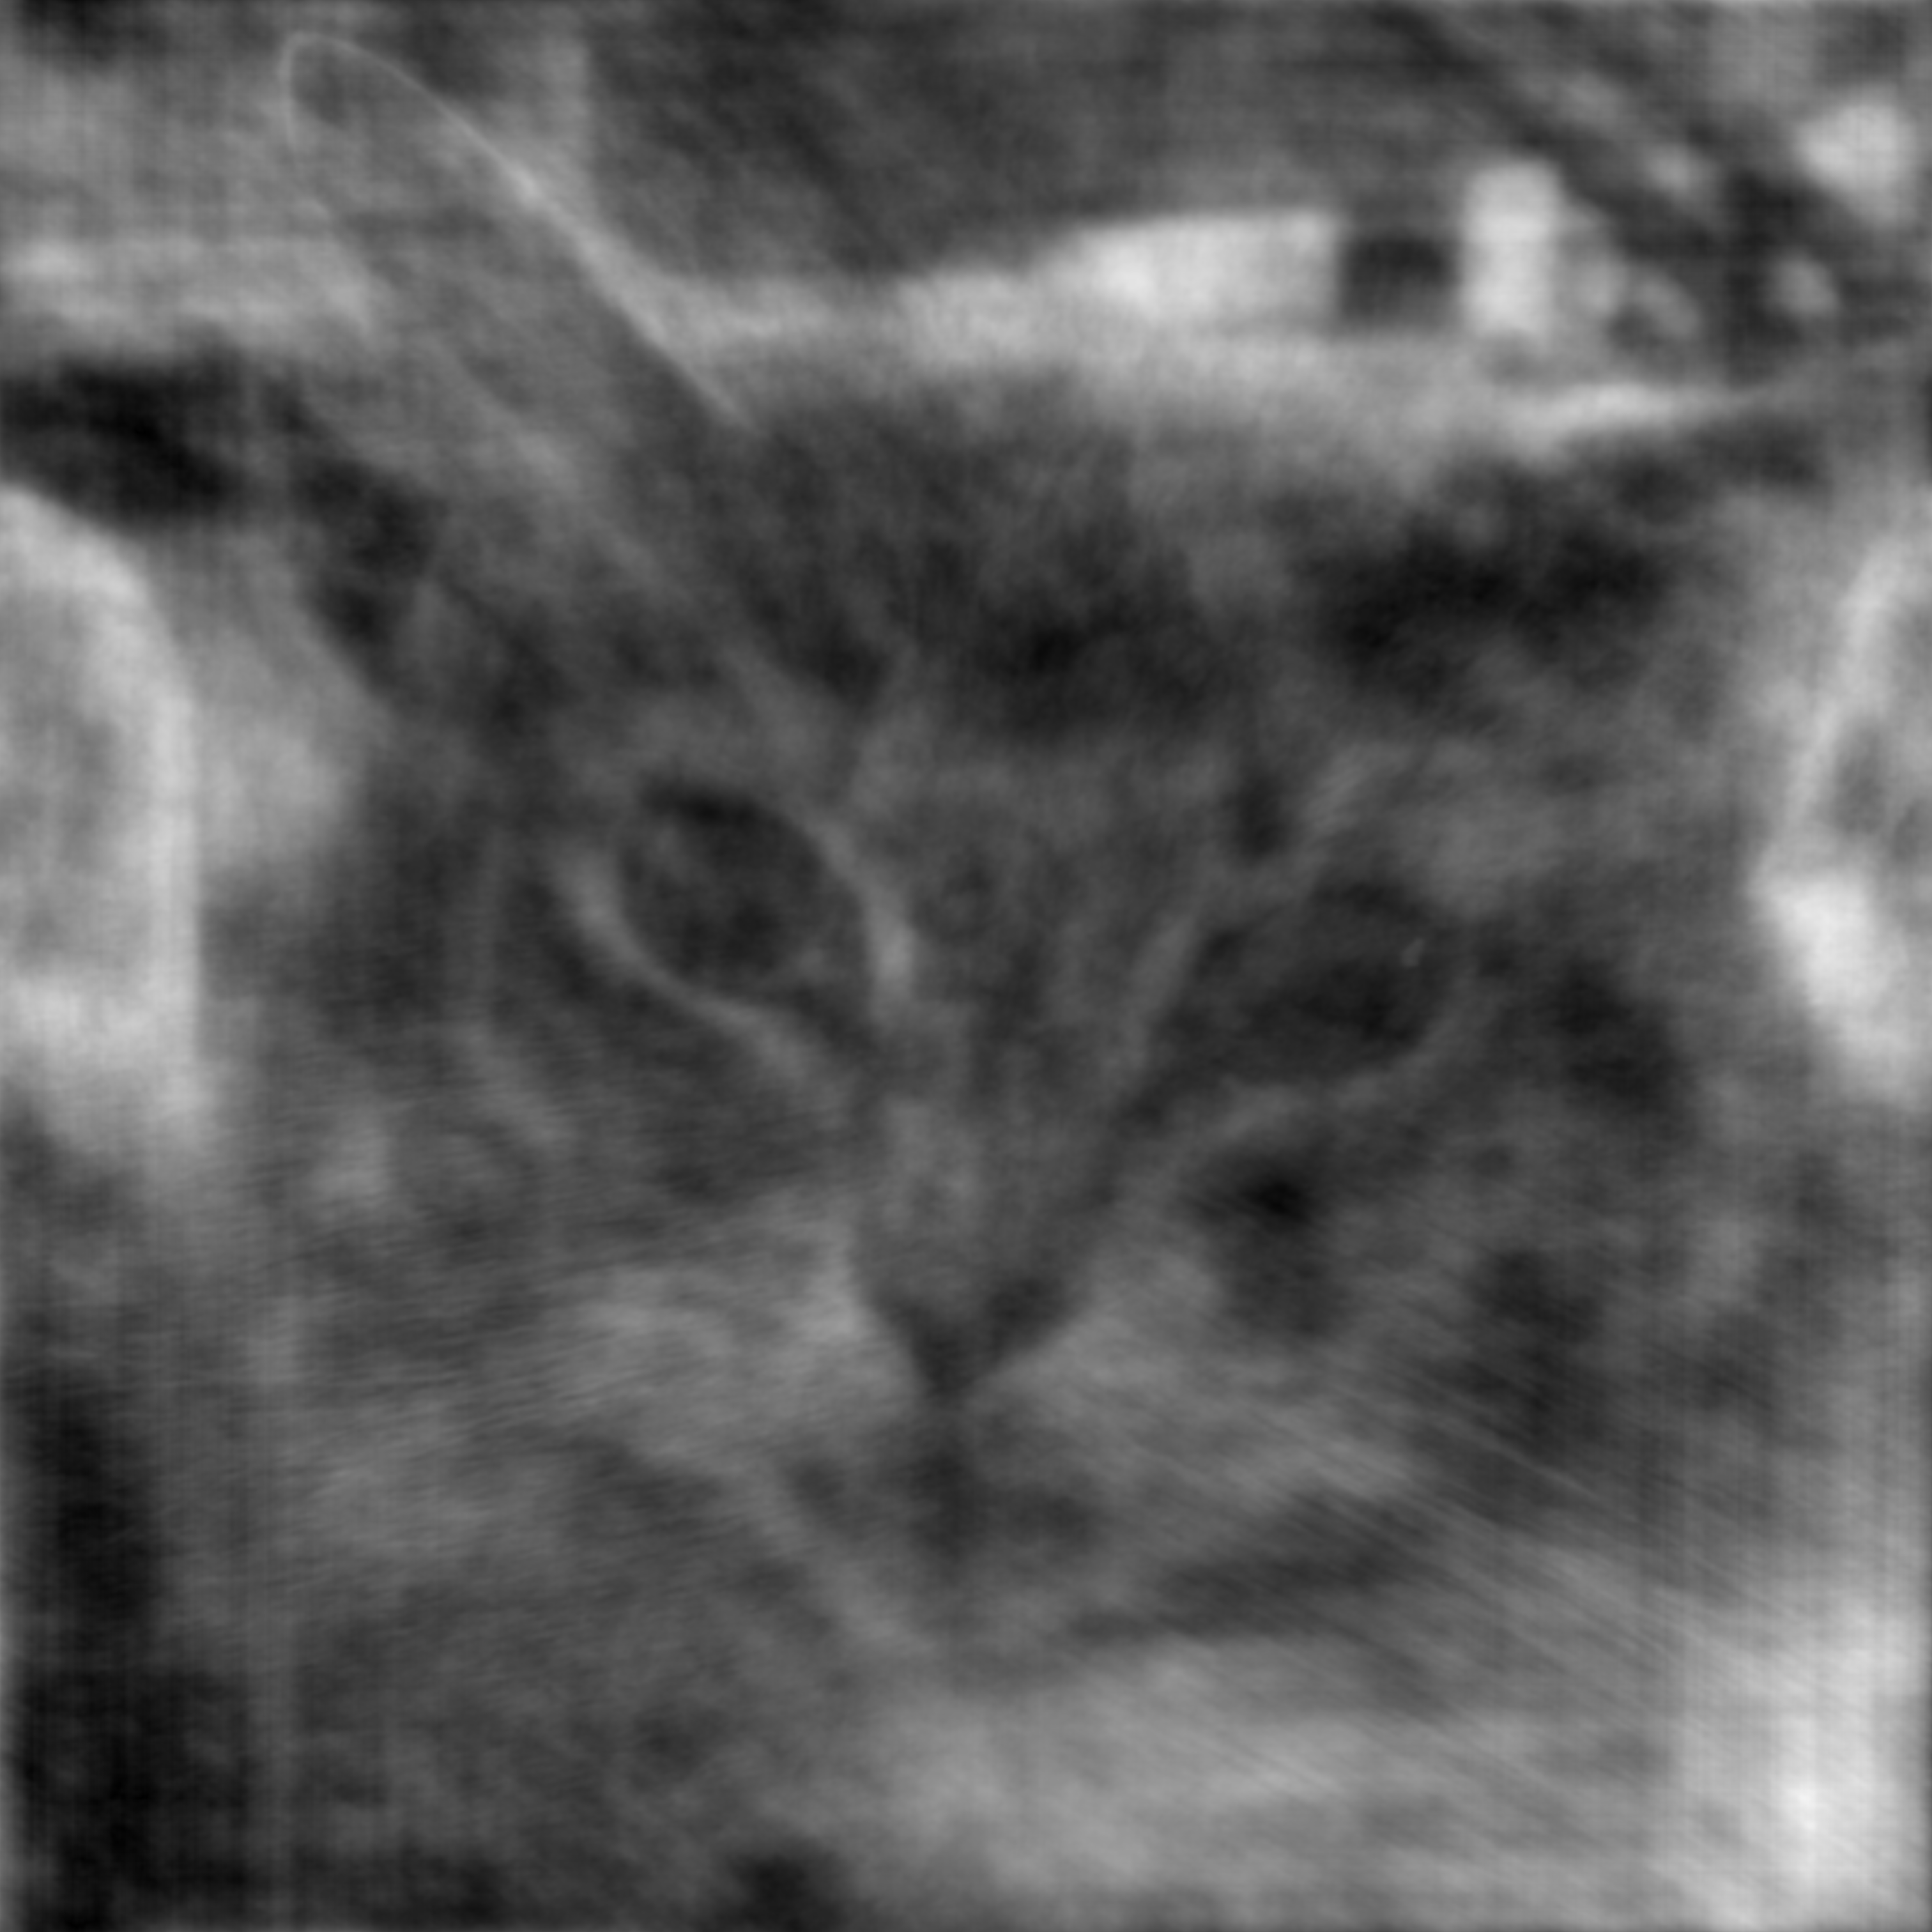
\includegraphics[height=4cm]{figures/dirty_image.png}} \\
        
        \multicolumn{5}{c}{\scalebox{1.5}{$\uparrow\mathcal{F}\downarrow$}} \\

        \subfloat[True Visibilities]{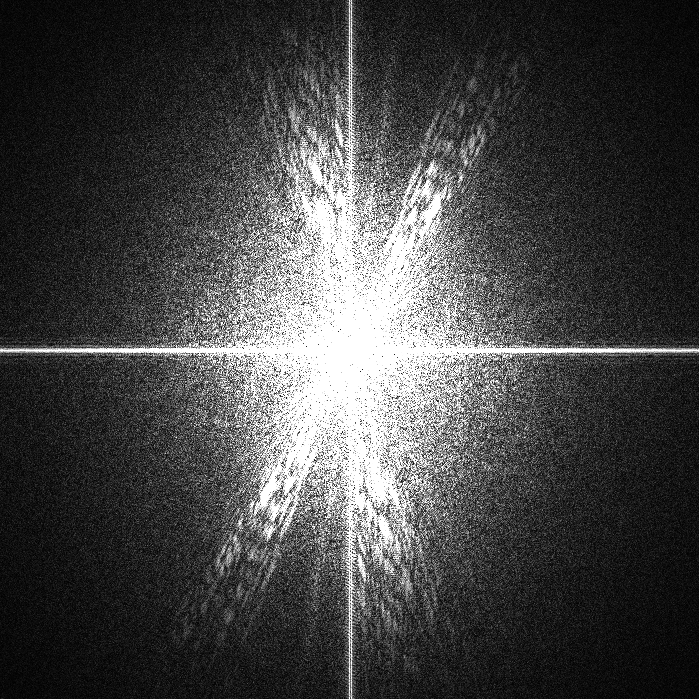
\includegraphics[height=4cm]{figures/true_response.png}} &
        \raisebox{1.84cm}{$\scalebox{1.5}{$\times$}$} &
        \subfloat[Sampling Function]{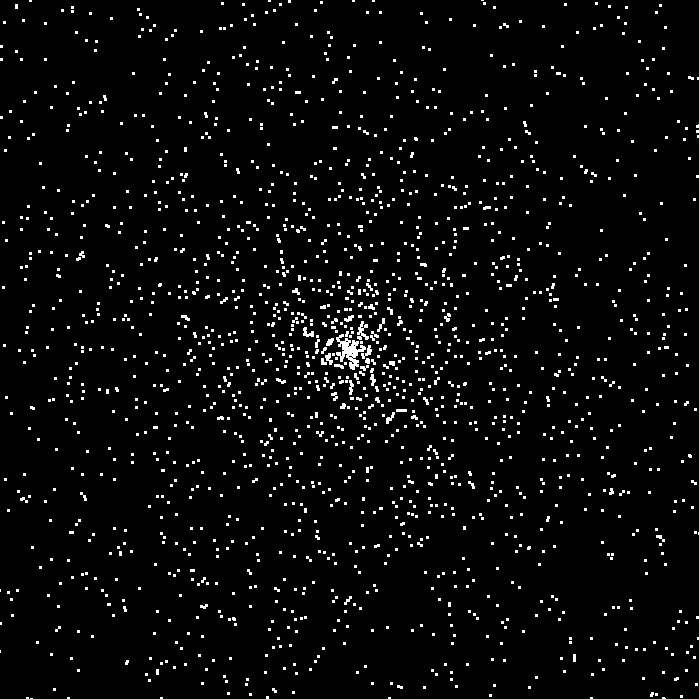
\includegraphics[height=4cm]{figures/sample_fun.png}} &
        \raisebox{1.84cm}{$\scalebox{1.5}{$=$}$} &
        \subfloat[Sampled Visibilities]{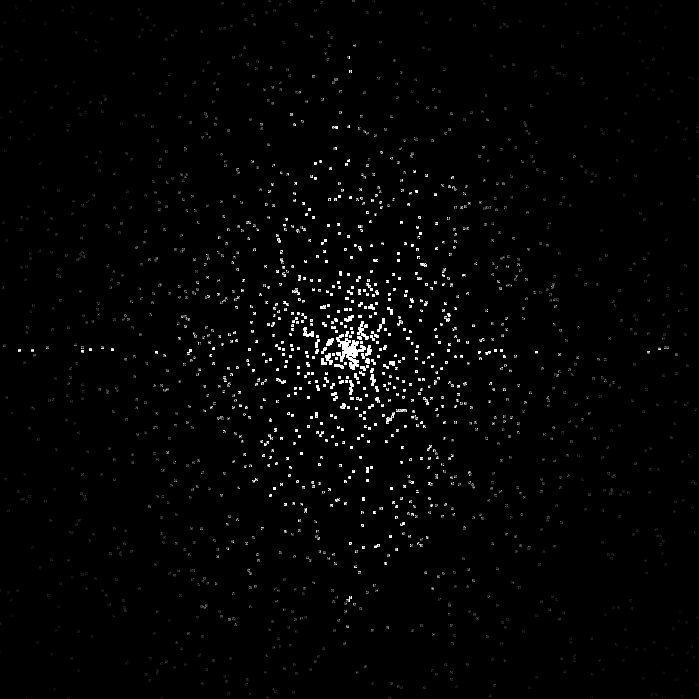
\includegraphics[height=4cm]{figures/sampled_response.png}} \\
    \end{tabular}
    \caption{Radio interferometer Fourier pairs}
    \label{fig:radio_imaging}%
\end{figure}

As we increase the number of antennas and the area they cover, we fill out the $uv$ plane more and more, resulting in a better image.
In the same manner as survey speed, this encourages us to build a telescope with bigger $N$.
However, the tradition in radio astronomy is to distribute the raw visibilities as the data product.
In sparse arrays like the Very Large Array, or the Event Horizon Telescope, the scientist performing the analysis might want full control over how the image is formed from the sparse data, making their own assumptions on how to interpret them.
For DSA-2000, let us assume we observe \num{16000} frequency channels every \num{10} seconds.
If there are \num{2000} dual-polarized antennas and each visibility is an 8+8-bit complex number, that works out to a visibility data rate of \num{25.6} GB per second.
Over a year at this rate, we would accumulate \num{0.8} exabytes of data\footnote{Or eight times the storage capacity of Data from Star Trek: The Next Generation}.
The entirety of the Internet Archive\footnote{\url{https://archive.org/}} stores around \num{100} petabytes of data for real-time, global access at a cost of \$2.5M per month.
At our data rate, that works out to \$300M per year, more than the construction cost of the array, just in storage!
Not only that, but this rate would keep increasing as we accumulate more and more data as we continue to survey the sky.
This cost is one of the primary reasons people have not built large arrays.

But here is the trick; at some point as $N$ increases, the $uv$ plane becomes complete enough where a simple inverse Fourier transform of the sampled visibilities results in a dirty image that requires little to no ``cleaning''.
Therefore, we could build a deterministic pipeline to capture images of the sky in real time and store those images instead of the raw visibilities, saving many orders of magnitude in storage costs.
This is what we call the ``Radio Camera'' concept and is the enabling feature of the DSA-2000, breaking the cost curve in storage for large $N$ arrays.
The low-pass filtering effect due to the maximum separation of antennas is still in play, resulting in less sharp final images.
This can be improved slightly through standard image post-processing such as sharpening algorithms or ML-based super resolution approaches~\cite{connorDeepRadiointerferometricImaging2022}.

\section{Thesis Outline}

Given the motivation to build an inexpensive, high-performance receiver, this thesis covers my work in squeezing out every drop of performance across the analog signal path for DSA-2000 to maximize sensitivity and survey speed, increasing our science impact per dollar.
The thesis is broken into two major sections, my work on the DSA-2000 and my work on the Galactic Radio Explorer (GReX), a separate, smaller experiment.
These are two distinct projects and are presented out of order chronologically, with DSA-2000 content presented first, representing the bulk of my work.
GReX acted as my introduction to the field of radio astronomy, starting early in my degree at Caltech.
It was intended to be a pathfinder instrument for DSA-2000, but changed in scope as the project progressed.

The novel contributions of this thesis are:
\begin{itemize}
    \item Development of an ambient-temperature low noise amplifier matching network using advanced algorithmic techniques (DSA-2000)
    \item Experiments with feed impedance to LNA noise matching and chip-scale Peltier micro-cooling (DSA-2000)
    \item Development of a low-cost, rapidly deployable radio telescope (GReX)
\end{itemize}

We start in \autoref{ch:lna_opt} with an overview of analytic formalisms surrounding low noise amplifier design and optimization.
Having a collection of closed-form results that encompass the various performance metrics for an LNA are required for designing an optimization framework.
\autoref{ch:lna} is a reproduction of an article that discusses the design of an improved room-temperature low noise amplifier for the DSA-2000, using the formalisms built in the previous chapter, and is my primary contribution.
\autoref{ch:asp} discusses the complete analog signal path for DSA-2000, including the analysis, design, and implementation of a high-performance RF over fiber link and further enhancements to the LNA such as solid-state cooling and antenna impedance co-optimization.
We finish with \autoref{ch:grex}, a reproduction of an article that describes the GReX instrument and new upper limits on galactic FRB populations.

\begin{figure}[h!]
    \centering
    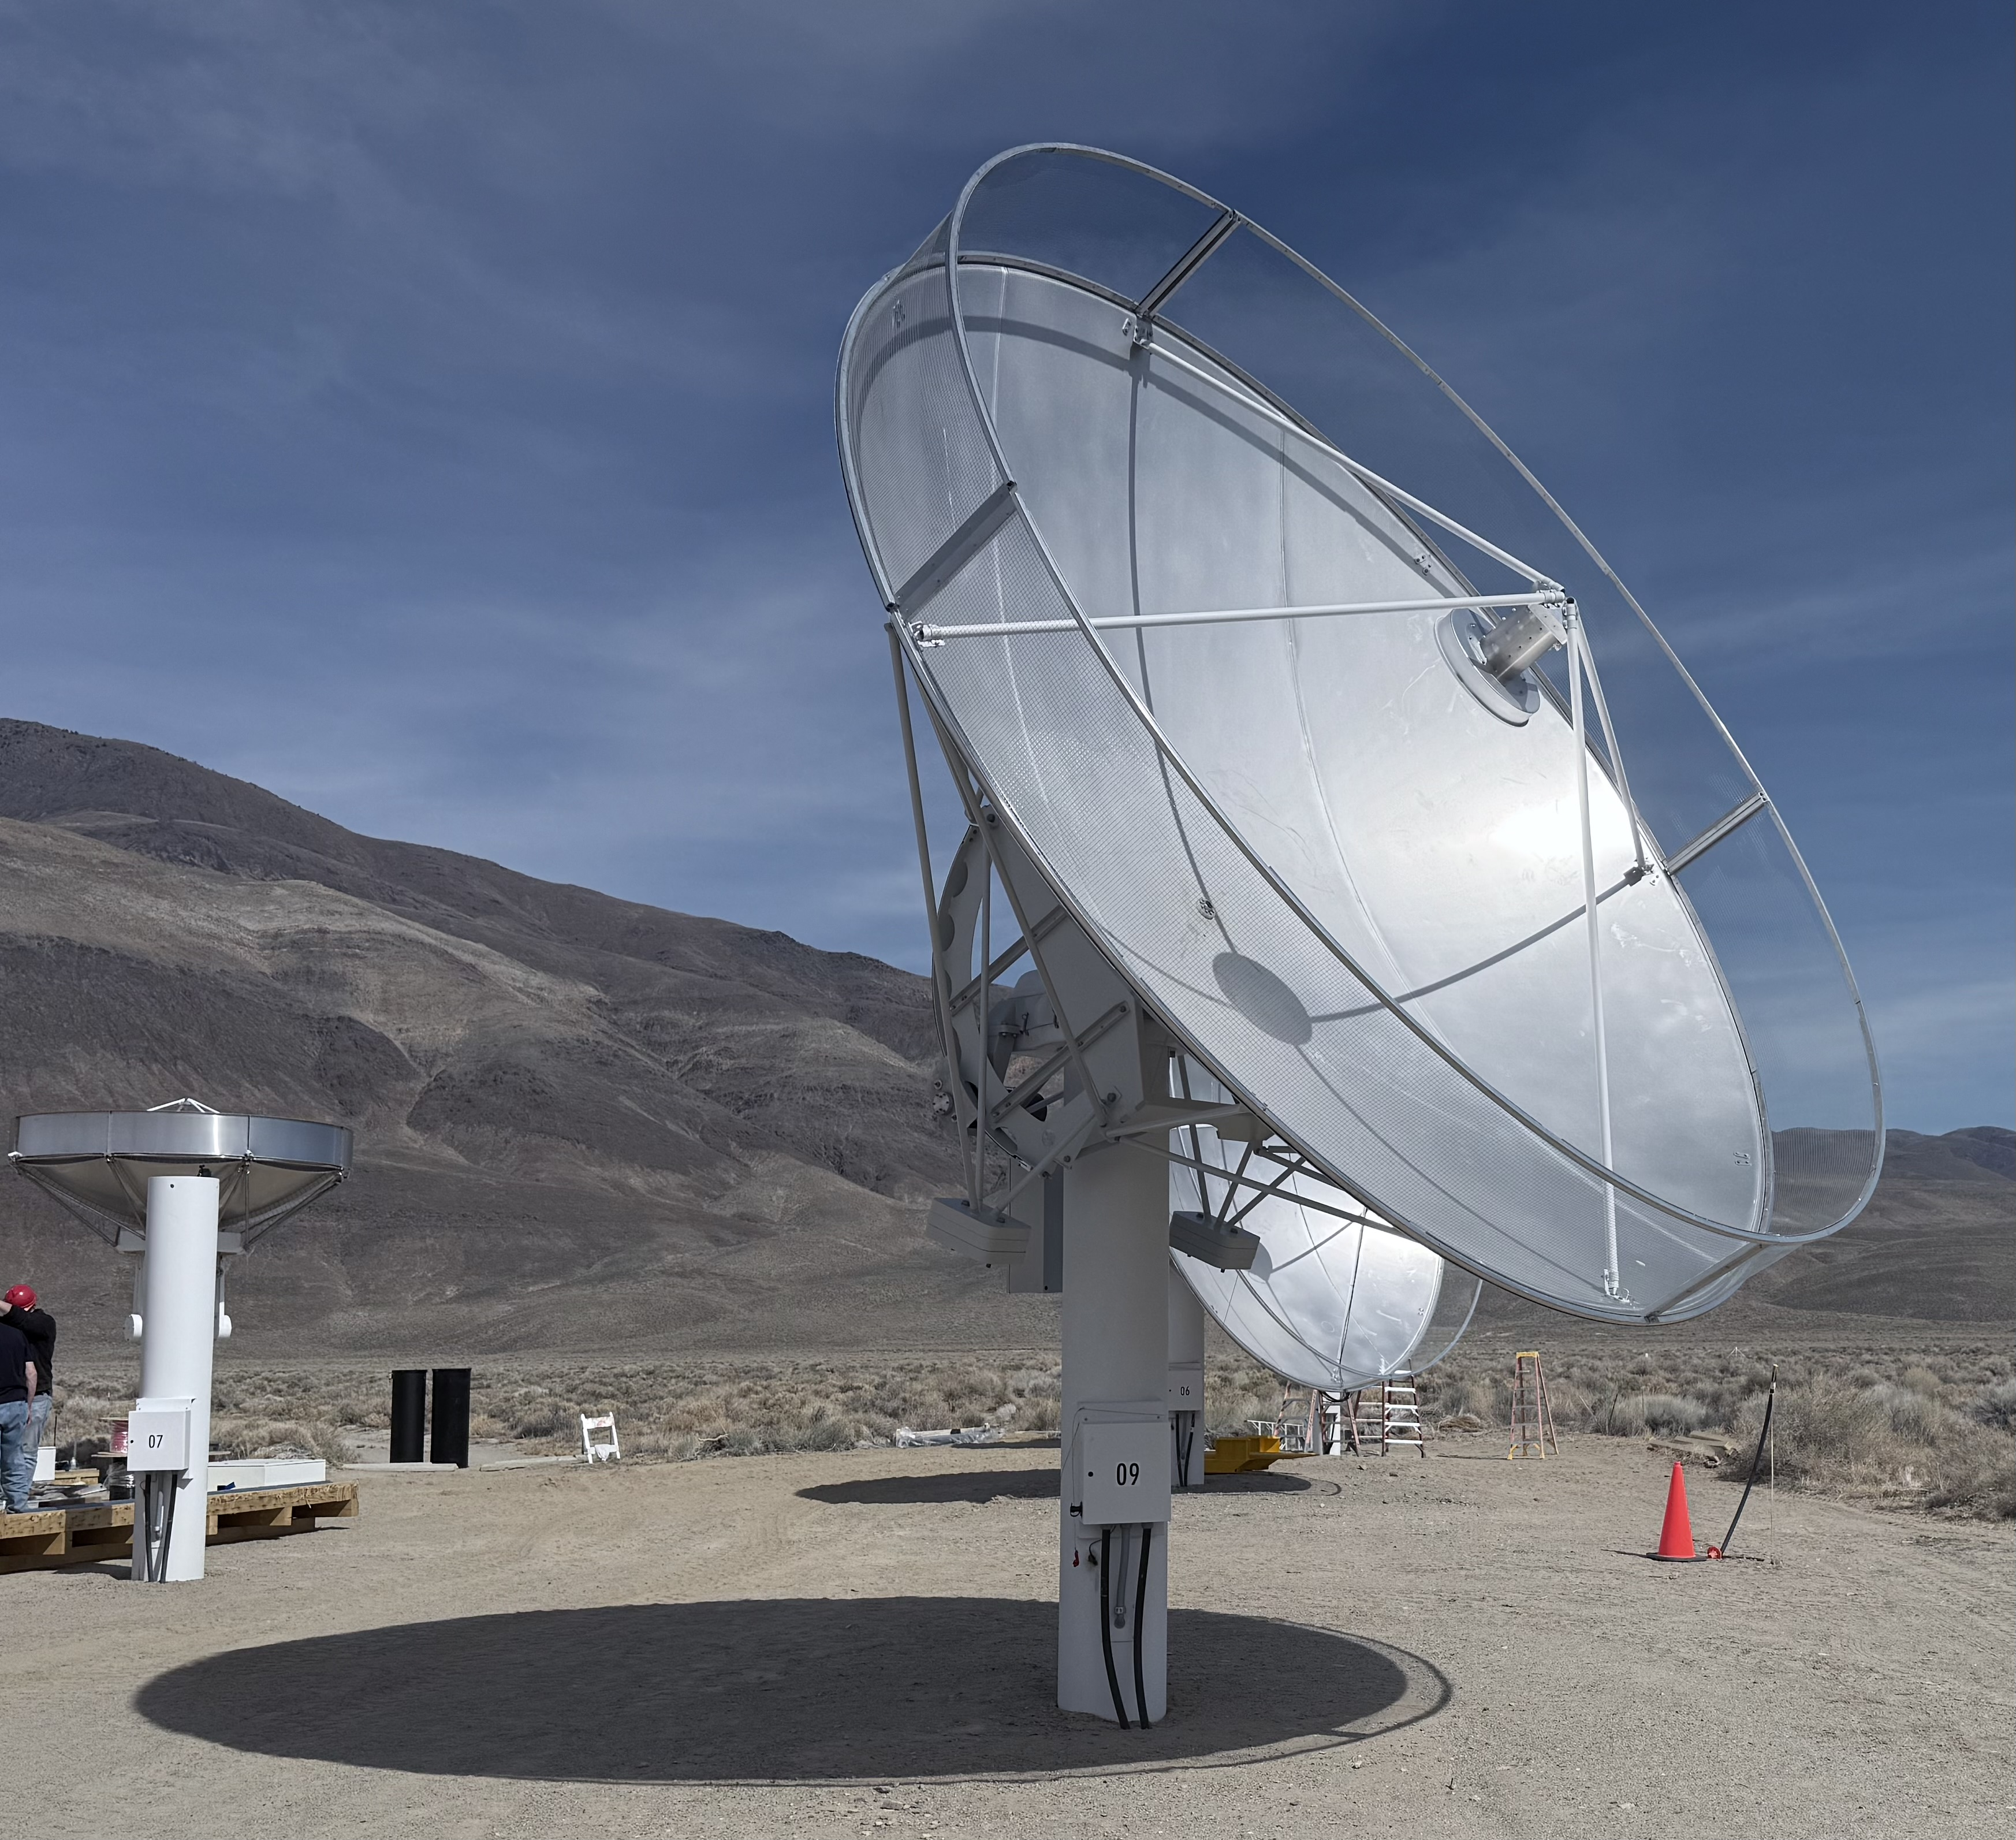
\includegraphics[width=\textwidth]{figures/test_array.jpg}
    \caption{DSA-2000 Test Array under construction at OVRO}
    \label{fig:test_array}
\end{figure}